\section{Introduction}%
\label{sec:introduction}%
%
\ac{DUS} is one of the safest forms of medical imaging and has become
ubiquitous in clinical practice, however it has been demonstrated to
trigger lung hemorrhage in a variety of animals. While the problem
does not appear to be one of significant medical concern under common
clinical conditions, the underlying cause is not well understood and
more information is needed so that future developments in ultrasound
remain safe. The purpose of this work is to investigate the underlying
physics of acoustically accelerated liquid-gas interfaces such as
those in the lungs. 

%
Over the last few decades \ac{DUS}-induced \ac{LH} has been
studied extensively and is the only known bioeffect of non-contrast,
pulsed \ac{US} known to occur in mammals. It has been demonstrated in
a variety of animal models including mice, rats, rabbits, pigs, and
monkeys \citep{Child1990,OBrien2006a,Tarantal1994a}. Presently the
physical damage mechanisms underlying the hemorrhage are not well
understood.

\ac{DUS}-induced \ac{LH} does not appear to be caused by traditionally
expected \ac{US} bioeffects mechanisms. Typically, \ac{US} bioeffects
mechanisms are classified as thermal or non-thermal with the bulk of
non-thermal bioeffects being a result of acoustic cavitation. Thermal
mechanisms have shown to be an unlikely cause of lung hemorrhage, as
\cite{Zachary2006} found that \ac{DUS}-induced lung lesions do not
appear similar to those induced by heat. There has also been
significant research suggesting that \ac{IC} is also an unlikely
damage mechanism for \ac{DUS}-induced \ac{LH} as \cite{OBrien2000}
observed that the severity of \ac{DUS}-induced \ac{LH} in mice
increased under raised hydrostatic pressure, and \cite{Raeman1996}
found that the hemorrhage is unaffected by the introduction of \ac{US}
contrast agents. One study reports detecting cavitation during
\ac{DUS}-lung interaction in rats \cite{Holland1996}. \cite{Tjan2007}
proposed that focused ultrasound may lead to the ejected of droplets
capable of puncturing the air-filled sacs within the lung, and
performed numerical simulations of as an inviscid, free surface
subjected to a Gaussian velocity potential to show that the proposed
droplet ejection may occur under certain circumstances. Similarly,
\cite{Simon2012} observed \ac{HIFU} induced atomization of tissue at
air interfaces. Despite these efforts, the precise damage mechanism
underlying \ac{DUS}-induced \ac{LH} is still unknown. And while
\ac{DUS} of the lung has not been observed to cause medical problems
in humans under typical clinical conditions, it is an important
problem to understand if we hope to further develop and improve
\ac{DUS} by expanding the physical regimes in which it operates.

Within the fluids community, there has been extensive research into
the fundamental physics describing interactions between mechanical
waves and fluid interfaces. However, much of this research is
motivated by applications in fusion energy and astrophysics and
accordingly has sought to investigate regimes outside of those of
acoustic interests. One topic of considerable past study is the
\ac{RMI}, in which a perturbed fluid-fluid interface is accelerated by
a shock, causing the interface perturbation to grow
\citep{Brouillette2002,Drake2006}. This growth is driven by a sheet of
baroclinic vorticity deposited along the interface as a result of
misalignment between the pressure gradient across the shock and the
density gradient across the perturbed interface. This physical
mechanism by which these misaligned gradients create a torque on fluid
particles and generate vorticity can be thought of in terms of a
hydrostatic balance upon a particle. Pressure gradients result in
acceleration of the flow. This acceleration is inversely proportional
to density. When these two gradients are misaligned, the result is a
shear stress on the fluid and vorticity is generated. An excellent
graphical explanation of this can be found in \cite{Heifetz2015}.
Analytically, baroclinic vorticity generation can be shown by taking
the curl of the conservation of momentum equation for a compressible
fluid. However we note that it is a nonlinear effect and cannot be
explained by traditional linear acoustics.
% \begin{figure}
%   \centering
%   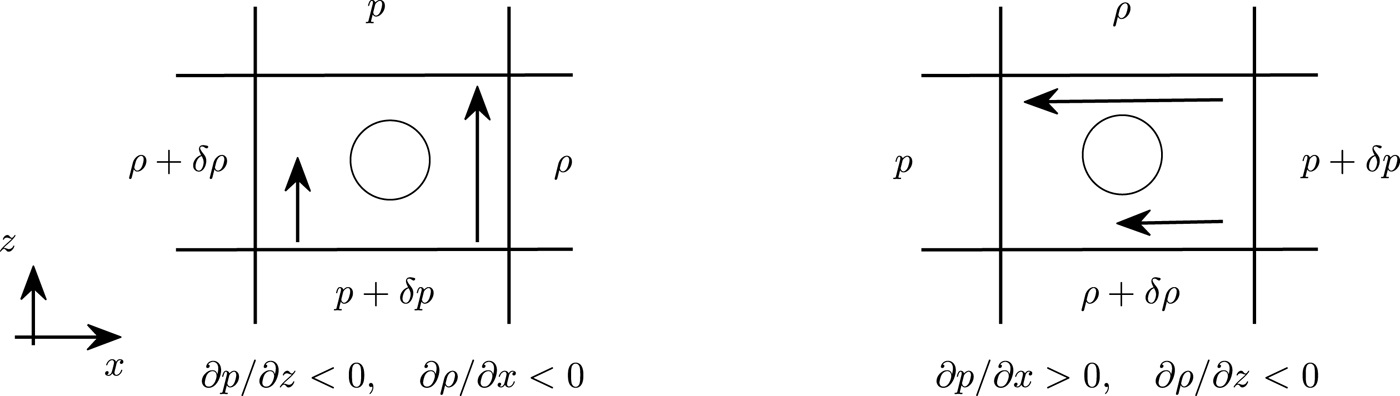
\includegraphics[width=0.9\textwidth]{./figs/lung_figs/baroclinic_schematic} \hfill
%   \caption[A schematic of baroclinic torque]{From
%     \cite{Heifetz2015}. A hydrostatic force balance upon a particle
%     subject to perpendicular pressure and density gradients
%     illustrates baroclinic torque on a fluid particle.}
%   \label{fig:usbe_lung_baroclinic_schematic}
% \end{figure}

The physics of the \ac{RMI} are fairly well understood. For the classical \ac{RMI}
setup a planar shock impinges normally upon the peaks and troughs of a
sinusoidal interface. As the degree of misalignment varies along the
interface, the interface is accelerated non-uniformly. The direction
of the vorticity changes where the slope of the interface
changes. This counter rotation on either side of interface peaks and
troughs entrains nearby fluid causing interface peaks to accelerate in
one direction and troughs to accelerate in the opposite
direction. This results in a ``bubble'' of light fluid penetrating the
heavy fluid, and a ``spike'' of heavy fluid penetrating the light
fluid. How exactly this occurs varies slightly depending on the
relative densities of the two fluids. For the case of a wave moving
from a light fluid into a heavy one, the peaks and troughs of the
interface are initially accelerated to move away from one another, and
the interface perturbation amplitude undergoes growth exclusively. For
the case of a wave moving from a heavy fluid to a lighter fluid, the
peaks and troughs of the interface are accelerated such that they
initially move closer to one another decreasing the perturbation
amplitude. They then pass one another, inverting the phase of the
interface perturbation, and then continue moving in opposite
directions, growing the perturbation amplitude. This process is
illustrated in Figure \ref{fig:rmi_schematic}, which has been adapted
from \cite{Brouillette2002}.
\begin{figure}
  \centering
  \def\svgwidth{0.9\textwidth}
  \import{./figs/lung_figs/}{brouillette_fig3_mod.pdf_tex} \hfill%
  \caption[A schematic view of the \ac{RMI} instability for a
  heavy-light interface]{Adapted from \cite{Brouillette2002}. The
    \ac{RMI} for a heavy-light interface is illustrated. The initial
    condition (left), circulation post wave-interface interaction
    (center), and perturbation growth (right) are shown.}
  \label{fig:rmi_schematic}
\end{figure}

Previous studies of the \ac{RMI} have utilized theory, computation, and
experiments to describe the behavior of the interface after the wave
has passed. \cite{Richtmyer1960} performed the linear stability
perturbation analysis developed by \cite{Taylor1950} for the case of
an impulsive acceleration to create a model for the initial growth of
the interface perturbation. \cite{Meshkov1969} experimentally
confirmed Richtmyer's qualitative predictions, hence the name of the
instability. \cite{Meyer1972} performed numerical simulations of the
\ac{RMI} and found good agreement with Richtmyer for the case of a
shock impinging upon a light-heavy interface. \cite{Fraley1986} used
Laplace transforms in order to find the first analytical solution for
the asymptotic growth rate for a shocked interface between perfect
gases. To describe the late time, nonlinear growth of the
perturbation, \cite{Zhang1997} used single mode perturbation, keeping
many high order terms, to describe the velocity of the bubble and
spike regions of the fluid. \cite{Sadot1998} combined the linear,
impulsive solution with potential flow models of the asymptotic
behavior of the bubble and spike to develop a model for the
perturbation growth that is in good agreement with shock tube
experiments for shocks with Mach numbers Ma=1.3, 3.5. Vortex theory
has also been used to describe the behavior of the
interface. \cite{Jacobs1996} horizontally oscillated a container with
two vertically stratified liquids to obtain standing waves and then
bounced the container off of a coil spring to study the incompressible
\ac{RMI}. The late time evolution of is interface is modeled using a
row of line vorticies to obtain qualitatively similar results to those
experimentally observed, however the late-time growth rate is
underestimated. \cite{Samtaney1994} used shock polar analysis to find
the circulation deposited by a shock on planar and non-planar
interfaces. Their results are validated using and Euler code and found
to be within 10\% of the computed value for $1.0\,<\,$Ma$\,\leq\,1.32$
for all $\rho_2/\rho_1\,>\,1$, and
$5.8\,\leq\,\rho_2/\rho_1\,\leq\,32.6$ for all Ma. This work aims to
add to the current body of work on this topic by investigating
interfaces accelerated by pressure waves within the acoustic regime.

% Accordingly we propose a possible damage mechanism of
% \ac{DUS}-induced \ac{LH}. We hypothesize that misalignment between
% the pressure gradients in the \ac{DUS} pulses and density gradients
% within the lungs create torque at the alveolar walls, which deform
% and ultimately hemorrhage as a result.

The detailed nonlinear interactions between acoustic waves and
perturbed liquid-gas interfaces do not appear to have been previously
studied in this manner or context. This work is separate from previous
research into the \ac{RMI} as a result of the acoustic regime
considered here. Unlike shock waves, which occur over a few molecular
mean free paths and interact nearly instantaneously, acoustic waves
have a finite spacial wavelength and can occupy a much larger portion
of space. Consequently, their interaction with interfaces occurs over
a longer period of time depending on the waveform and the geometric
and material properties of the media. This duration can also be
thought of in terms of the relative sizes of the physical features of
the interface and the wavelengths of each feature of the acoustic wave
of interest. Simple \ac{RMI} analysis assumes an impulsive
acceleration, and does not apply to this work because the interface
deforms throughout its interaction with the wave.

Additionally, we argue that the basic problem setup of the \ac{RMI}, a
mechanical wave impinging upon a material interface, has many
physical similarities to the motivating problem of \ac{DUS} of the
lungs. While the pressure gradient due to the \ac{US} pulse is not as
sharp as it would be across the shock, there is a strong density
discontinuity across the tissue-air interfaces of the
lungs. Accordingly, we study problem geometries and acoustic waves
within the regimes of \ac{DUS} of the lung.

In the remainder of this work we will first present a model problem
and a set of numerical experiments designed to investigate the
fundamental physics underlying interactions between acoustic waves and
perturbed interfaces between fluids. We will present results that
specifically explore the dependence of the interface dynamics on
acoustically relevant properties including the amplitude and
wavelength of the acoustic wave. We pay particular attention to the
finite duration of the wave-interface interaction, and the interface
deformation that occurs during this period. We perform analysis to
explain the vorticity deposition and late time behavior of the
interface after all acoustic waves have passed. The results will be
discussed to address the following questions:
\begin{enumerate} \label{itm:usbe_lung_questions}
\item Are acoustic waves capable of generating sufficient baroclinic
  vorticity at perturbed liquid-gas interfaces for substantial
  deformations?
\item What is the impact of the acoustic wave properties, such as
  amplitude and wave duration, on the vorticity and interface
  dynamics?
\end{enumerate}
We will then discuss on the significance of these results as
they regard to the motivating problem of \ac{DUS}-induced lung
hemorrhage. We will finally end by summarizing the main conclusions
drawn from this work and suggest the next steps to be taken.



% \hl{ (MOVE ALL THIS TO LATER)
% We consider a compressible multi-fluid system and
% solve the Euler equations of inviscid fluid motion to study the
% dynamics of fluid-fluid interfaces exposed to acoustic waves relevant
% to \ac{DUS}. We observe that acoustically-generated vorticity at
% perturbed water-air interfaces drives the interface to deform. We
% hypothesize that a similar mechanism may be responsible for deforming
% and ultimately rupturing the fragile tissue barriers around alveoli,
% tiny air sacs within the lungs, leading to \ac{DUS} induced \ac{LH}.}




%%% Local Variables:
%%% mode: latex
%%% TeX-master: "../main"
%%% End:
